\begin{frame}
	\frametitle{Amostragem, quantização e o formato do arquivo \textit{Wave}}
	\begin{columns}
		\column{0.6\textwidth}
		\begin{figure}
			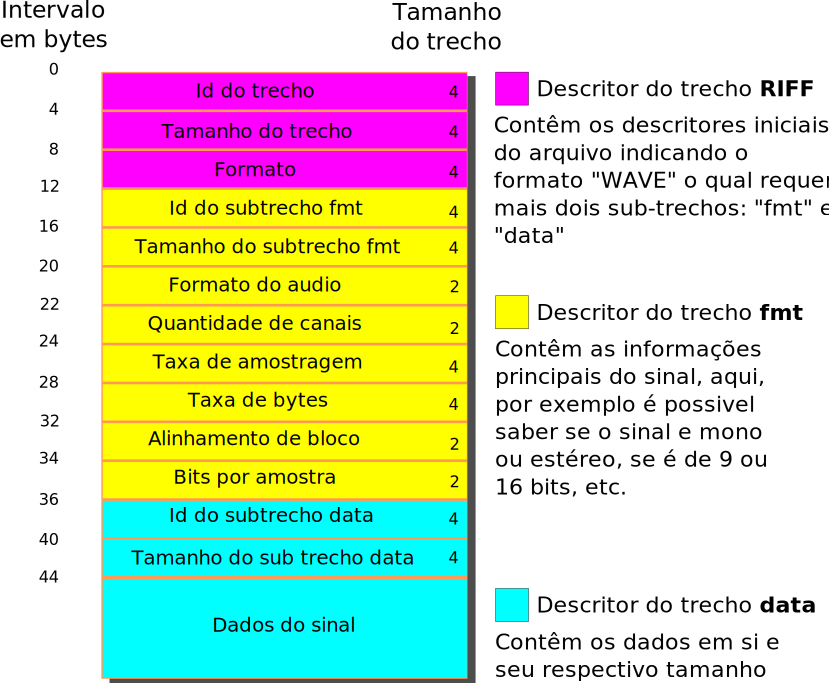
\includegraphics[width=.8\linewidth, angle=-90]{../monography/images/wavePcmStructure.pdf}
			\label{fig:wavePcmStructure}
		\end{figure}
		\column{0.4\textwidth}
		\begin{itemize}
			\item Formato \textit{wave}.
			\item \textit{Pulse-code modulation} (PCM).
			\item Taxa de amostragem de 44100hz.
			\item Resolução de 16bits
		\end{itemize}
	\end{columns}
\end{frame}